\chapter{Discussion} % Main chapter title

\label{Chapter:Discussion}

\section{Urban agriculture-sustainable city nexus}

Based on the theory of ‘highest and best use’ of land, authorities of cities across the globe prefer to zone urban lands for non-agricultural purposes. This is underpinned by the perception that agriculture in cities does not promote the highest and best use of city land due to its low bid-rent. Consequently, agriculture has been priced out of the city landscape, at a period where the clarion call for sustainable cities has been loud. Some scholars maintain that pricing out agriculture from a city landscape undermines its sustainability efforts in terms of economic, social and ecological functions \cite{Binns2013, Prain2010, Ackerman2014, Opitz2016, Specht2014} (Dimitri, Oberholtzer, \& Pressman, 2016; McLees, 2016; Obach \& Tobin, 2014; Pole \& Gray, 2013). Other scholars refute agriculture's role in the sustainability of cities (Edet \& Etim, 2013; International Labour Organization, 2006; Obuobie et al., 2006; Veenhuizen, 2006; Yamusa, 2014). To this group of authors, the roles of urban agriculture in sustainable cities have been exaggerated. Some of the agricultural practices even undermine the sustainability efforts of cities while the positive roles are not significant enough to contribute to sustainable cities. Based on the ongoing debate, the purpose of this review paper was to attempt to clarify the nexus between urban agriculture and sustainable cities.

The results of the review indicate that the urban agriculture-sustainable city nexus manifests in economic, social and ecological terms. From the economic perspective, urban agriculture contributes to fulltime employment (including employment for women), income generation, savings, capital spending, and tax revenue. Its unbiased nature, in terms of employment creation and savings for both males and females \cite{Prain2010}, has positive implications for gender equality and social equity. However, these economic benefits, measured in terms of full-time employment, household and city income, and capital spending, could have been higher if the prime lands used for agriculture were used for non-agricultural purposes such as commercial, industrial or residential. For instance, with reference to the Alonso's bid-rent theory, commercial and industrial land uses can offer higher rents for a parcel of land acquired and used for these purposes. Furthermore, non-agricultural land uses in cities may make more profound contributions to employment creation and capital expenditure than urban crop farming despite its labour-intensive character. The high land rent and job creation may have positive implications for a city's income through taxation.

Urban agriculture's roles in food security in cities appear to have been exaggerated (Frayne, Mccordic, \& Shilomboleni, 2014). For instance, some scholars \cite{Amponsah2016a} (Astee \& Kishnani, 2010) claim that this exaggeration is because of vegetables and herbs being the dominant produce from the sub-sector. The narrative in the conventional literature suggests that the calorie content of vegetables and herbs is low (Darmon, Darmon, Maillot, \& Drewnowski, 2005) for which reason they are associated with lower risks of chronic diseases (Wadhera, Capaldi Phillips, \& Wilkie, 2015). In this regard, the vegetables and herbs can only perform supplementary roles in food security. The discussion, therefore, indicates that urban agriculture loses the debate in the economic sustainability of cities, especially when compared with land uses such as commercial, industrial and residential whose bid-rents are higher. This could explain city authorities' low affinity for agricultural land uses in city landscapes (Nugent, 2000).

However, the economic sustainability analyses are only based on the direct benefits of urban agriculture and disregard its ecological functions. For instance, the waste management functions of urban agriculture not only promote environmental quality but also create employment for those who produce compost from municipal waste for use in the urban farms. Furthermore, the emission management roles of urban agriculture (Chen et al., 2013; Heather, 2012; Padgham et al., 2015; Yang et al., 2008) contribute to making cities liveable. Urban agriculture's roles in sustainable cities are further evident in its profound roles in water management (Richman, 2015; Vyawahare, 2016) and energy-efficiency functions (Gill et al., 2007; Guo-yu et al., 2013; Voiland, 2010).

Karl Marx, in his theory of metabolic rift, argued that “large landed property produces conditions that provoke an irreparable rift in the interdependent process of social metabolism, which is prescribed by the natural laws of life” (Marx, 1981). In this vein, urban agriculture, through its ecological functions, can help to mitigate the adverse effects of commercial, industrial and residential investments on cities physical environment. This underscores the importance of urban agriculture to the sustainability of cities. These environmental functions are not considered in the discourse on the role of urban agriculture in economic sustainability of cities mainly because quantifying the economic benefits of the environmental services appears to be a daunting task. Therefore, the implication is that the conclusions on the role of urban agriculture in the sustainable city discourse appear to be based on incomprehensive analysis of its roles in city sustainability. Researchers must therefore be cautious when using cost-benefit analysis to assess the benefits derived from urban agriculture since it can grossly be under estimated (Takyi \& Seidel, 2017).

Its social roles further consolidate its position in the city sustainability discourse. These social roles include education (Bradley \& Galt, 2014; Golden, 2013; Ober Allen et al., 2008; Travaline \& Hunold, 2010); safety and security \cite{Hoornweg2012} (Krauser, 2012; Rashid \& Ahmed, 2011; Wong et al., 2003); human health \cite{Opitz2016} (Golden, 2013; Twiss et al., 2003; World Bank, 2013); recreation (Hamilton et al., 2013; Walker, 2015); and technology and innovation (Buehler \& Junge, 2016; Close et al., 2006; Woodford, 2018). However, these roles are seldom quantified and included in the valuation of the benefits of urban agriculture in the sustainable city discourse.

From the discussion, we point out that the discourse on the role of urban agriculture in the sustainability of cities should not focus on only the economic dimension of sustainability but consider the social and environmental dimensions together with the economic benefits. Concluding only on the economic benefits is a travesty of the whole idea of sustainable development.

\section{Implications for cities in the global south and compact cities}

The narrative suggests that the cities in the global south are the worst culprits in pricing out agriculture from the city landscape (see: Cobbinah \& Niminga-Beka, 2017; Kuusaana \& Eledi, 2015). The authorities of these cities should make spaces available for urban agriculture. These spaces should be acquired from the owners and be zoned for agricultural purposes. The justification lies in the social and ecological functions of urban agriculture. Furthermore, the riparian areas that are often avoided by developers in developing countries due to their marginal nature and the high cost of their development should be zoned for urban agricultural purposes. For instance, in Ghana, these areas are already in use by urban farmers who produce vegetables for the growing population of vegetable consumers \cite{Amponsah2015, Amponsah2016} (Orsini, Kahane, Nono-Womdim, \& Gianquinto, 2013). Wetland farming is also a major source of livelihood for farmers in Rwanda although that poses several challenges to its ecological functions (Nabahungu \& Visser, 2011). However, farming practices that completely change the landscape from the use of inorganic farming practices undermine the ecological functions of the riparian areas. Organic rice farming in these riparian areas could be ideal strategy to sustaining the ecological uses of these riparian areas (Lawler, 2004). Planting commercial trees in these areas can also be an important strategy to cleaning the urban environment. The lands must be acquired by paying the right amount of compensations to the landowners. This will ensure their continued use for agricultural purposes.

Compact cities are much more focused on intensification, consolidation or densification, particularly around inner suburbs (Abdullahi et al., 2015). A shift from land-intensive urban agricultural practices to soil-free and less land intensive agricultural practices could be the ideal pathway to sustaining urban agriculture in these cities. Models such as roof-top gardening, film farming, aeroponic, hydroponic and sack farming would not only sustain urban farming but also ensure water and energy use efficiency as well as guarantee the health of the stakeholders along the value chain due to the limited agro-chemicals (Joe, 2017; Vyawahare, 2016; Woodford, 2018). These farming models do not require soil, hence their suitability for cities that are bedevilled by land scarcity. Film farming, for instance, is practiced across 180 farms in Japan and has been tested in China, Pakistan, Nigeria, and the United Kingdom. Sack farming has also been successful in Kenya, Uganda, Bangladesh (Peprah, Amoah, \& Akongbangre, 2014). The implication of the study is that the city land use planning process and building permitting process in developing countries need to be reviewed to accommodate these models of urban agricultural practices.

%\begin{figure}[th]
%\centering
%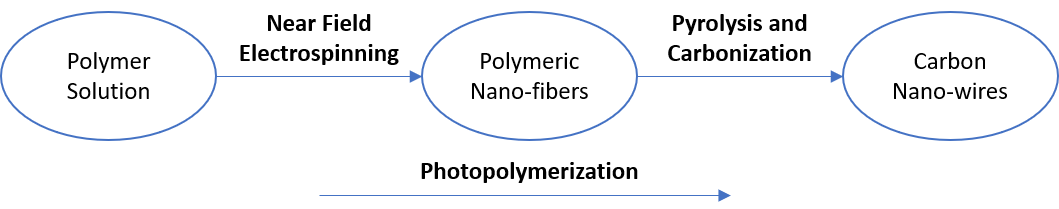
\includegraphics[width=0.95\textwidth]{./Figures/FabricationProcess.png}
%\decoRule
%\caption[Carbon Nano-wires Fabrication Process]{Fabrication process of carbon nano-wires to achieve through the proposed dissertation.}
%\label{fig:fabricationFlowChart}
%\end{figure}

%\begin{equation}
%\left(\tau _t^e-\frac{\tau _n^e \text{dr}}{\text{dz}}\right) 2 \pi  r+\frac{d \left(\pi  r^2
%   \left(\tau _{\text{zz}}-p\right)\right)}{\text{dz}}+\frac{\gamma  \text{dr} 2 \pi  r}{r
%   \text{dz}}+\rho  g \pi  r^2=\frac{d \left(\rho  \pi  r^2 v^2\right)}{\text{dz}}
%\label{eq:linearMomentum}
%\end{equation}